\documentclass{beamer}
\usetheme{pnl}
\usepackage[utf8]{inputenc}
\usepackage[T1]{fontenc}
\usepackage{hyperref}
\usepackage{tikz}
\usetikzlibrary{positioning}

\graphicspath{{img/}}

\usepackage{listings}
\usepackage{xcolor}

\definecolor{codegreen}{rgb}{0,0.6,0}
\definecolor{codegray}{rgb}{0.5,0.5,0.5}
\definecolor{codepurple}{rgb}{0.58,0,0.82}
\definecolor{backcolour}{rgb}{0.95,0.95,0.92}

\lstdefinestyle{mystyle}{
    backgroundcolor=\color{backcolour},   
    commentstyle=\color{codegreen},
    keywordstyle=\color{magenta},
    numberstyle=\tiny\color{codegray},
    stringstyle=\color{codepurple},
    basicstyle=\ttfamily\footnotesize,
    breakatwhitespace=false,         
    breaklines=true,                 
    captionpos=b,                    
    keepspaces=true,                 
    numbers=left,                    
    numbersep=5pt,                  
    showspaces=false,                
    showstringspaces=false,
    showtabs=false,                  
    tabsize=2
}

\lstset{style=mystyle}

\title{Practice Big Data-NET17237}
\date[8-9-2022]{Instalasi}
\author[Davi]{Muhammad Davi, S.Kom., M.Cs.\\ 
\texttt{muhammad.davi@pnl.ac.id}\\ 
\texttt{\small 14-9-\the\year{}}}

\begin{document}

\tikzset{
	phase/.style={draw,minimum width=1cm,minimum height=1cm,align=center},
	previous/.style={below right=0.1cm of #1}
}
  
\newcommand\connect[2]{
	\draw[->,thick] (#1) -| (#2);
	\draw[->,thick] (#2) -| (#1);
}
  
\begin{frame}[t]
\titlepage
\end{frame}

\begin{frame}[t]
\frametitle{Outline}
\begin{itemize}
\item Install Java
\item Install Hadoop
\item Running Hadoop
\item Code
\end{itemize}
\end{frame}

\begin{frame}[t]
\frametitle{Install Java}
\framesubtitle{Instalasi}
\begin{itemize}
\item Install Java
\begin{itemize}
\item sudo apt update
\item sudo apt install openjdk-8-jdk -y
\end{itemize}
\item Verifikasi Java
\begin{itemize}
\item java -version
\end{itemize}
\end{itemize}
\end{frame}

\begin{frame}[t]
\frametitle{Install Hadoop}
\framesubtitle{Instalasi}
\begin{itemize}
\item Buat folder
\begin{itemize}
\item mkdir $\sim$/hadoop
\end{itemize}
\item Pindah ke folder hadoop
\begin{itemize}
\item cd hadoop
\end{itemize}
\item Download Hadoop \href{https://hadoop.apache.org/releases.html}{(https://hadoop.apache.org/releases.html)}
\begin{figure}
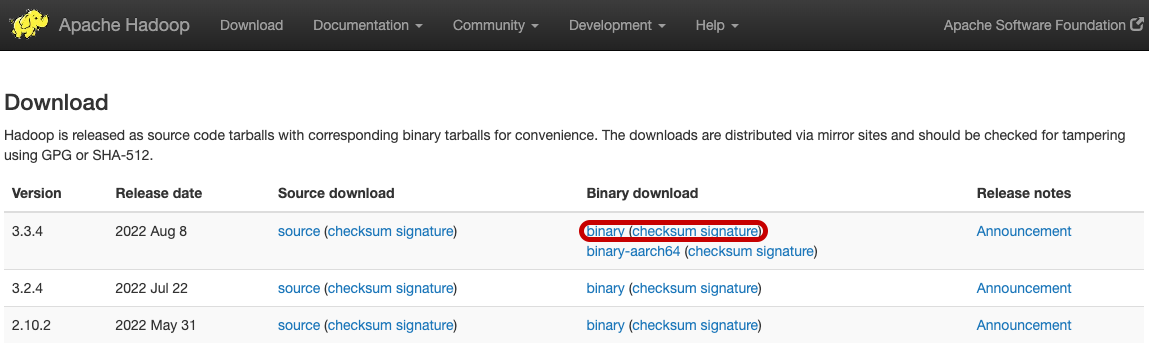
\includegraphics[scale=.25]{download-hadoop-1.png}
\end{figure}
\end{itemize}
\end{frame}

\begin{frame}[fragile]
\frametitle{Running Hadoop}
\framesubtitle{Instalasi}
\begin{verbatim}
/usr/local/hadoop/bin/hadoop
\end{verbatim}
\end{frame}

\begin{frame}[fragile]
\frametitle{Code}
\framesubtitle{Instalasi}
\begin{lstlisting}[language=Python]
import numpy as np
    
def incmatrix(genl1,genl2):
    m = len(genl1)
    n = len(genl2)
    M = None #to become the incidence matrix
    VT = np.zeros((n*m,1), int)  #dummy variable
    
    #compute the bitwise xor matrix
    M1 = bitxormatrix(genl1)
    M2 = np.triu(bitxormatrix(genl2),1) 
\end{lstlisting}
\end{frame}

%thank you
\setbeamertemplate{background}{}
\setbeamertemplate*{lastpage}{}
\usebeamertemplate*{lastpage}

\end{document}
